% !TeX root = SketchFace.tex

\section{Deep Network for Sketch-Photo Translation}
\label{sec:network}

\begin{figure*}
	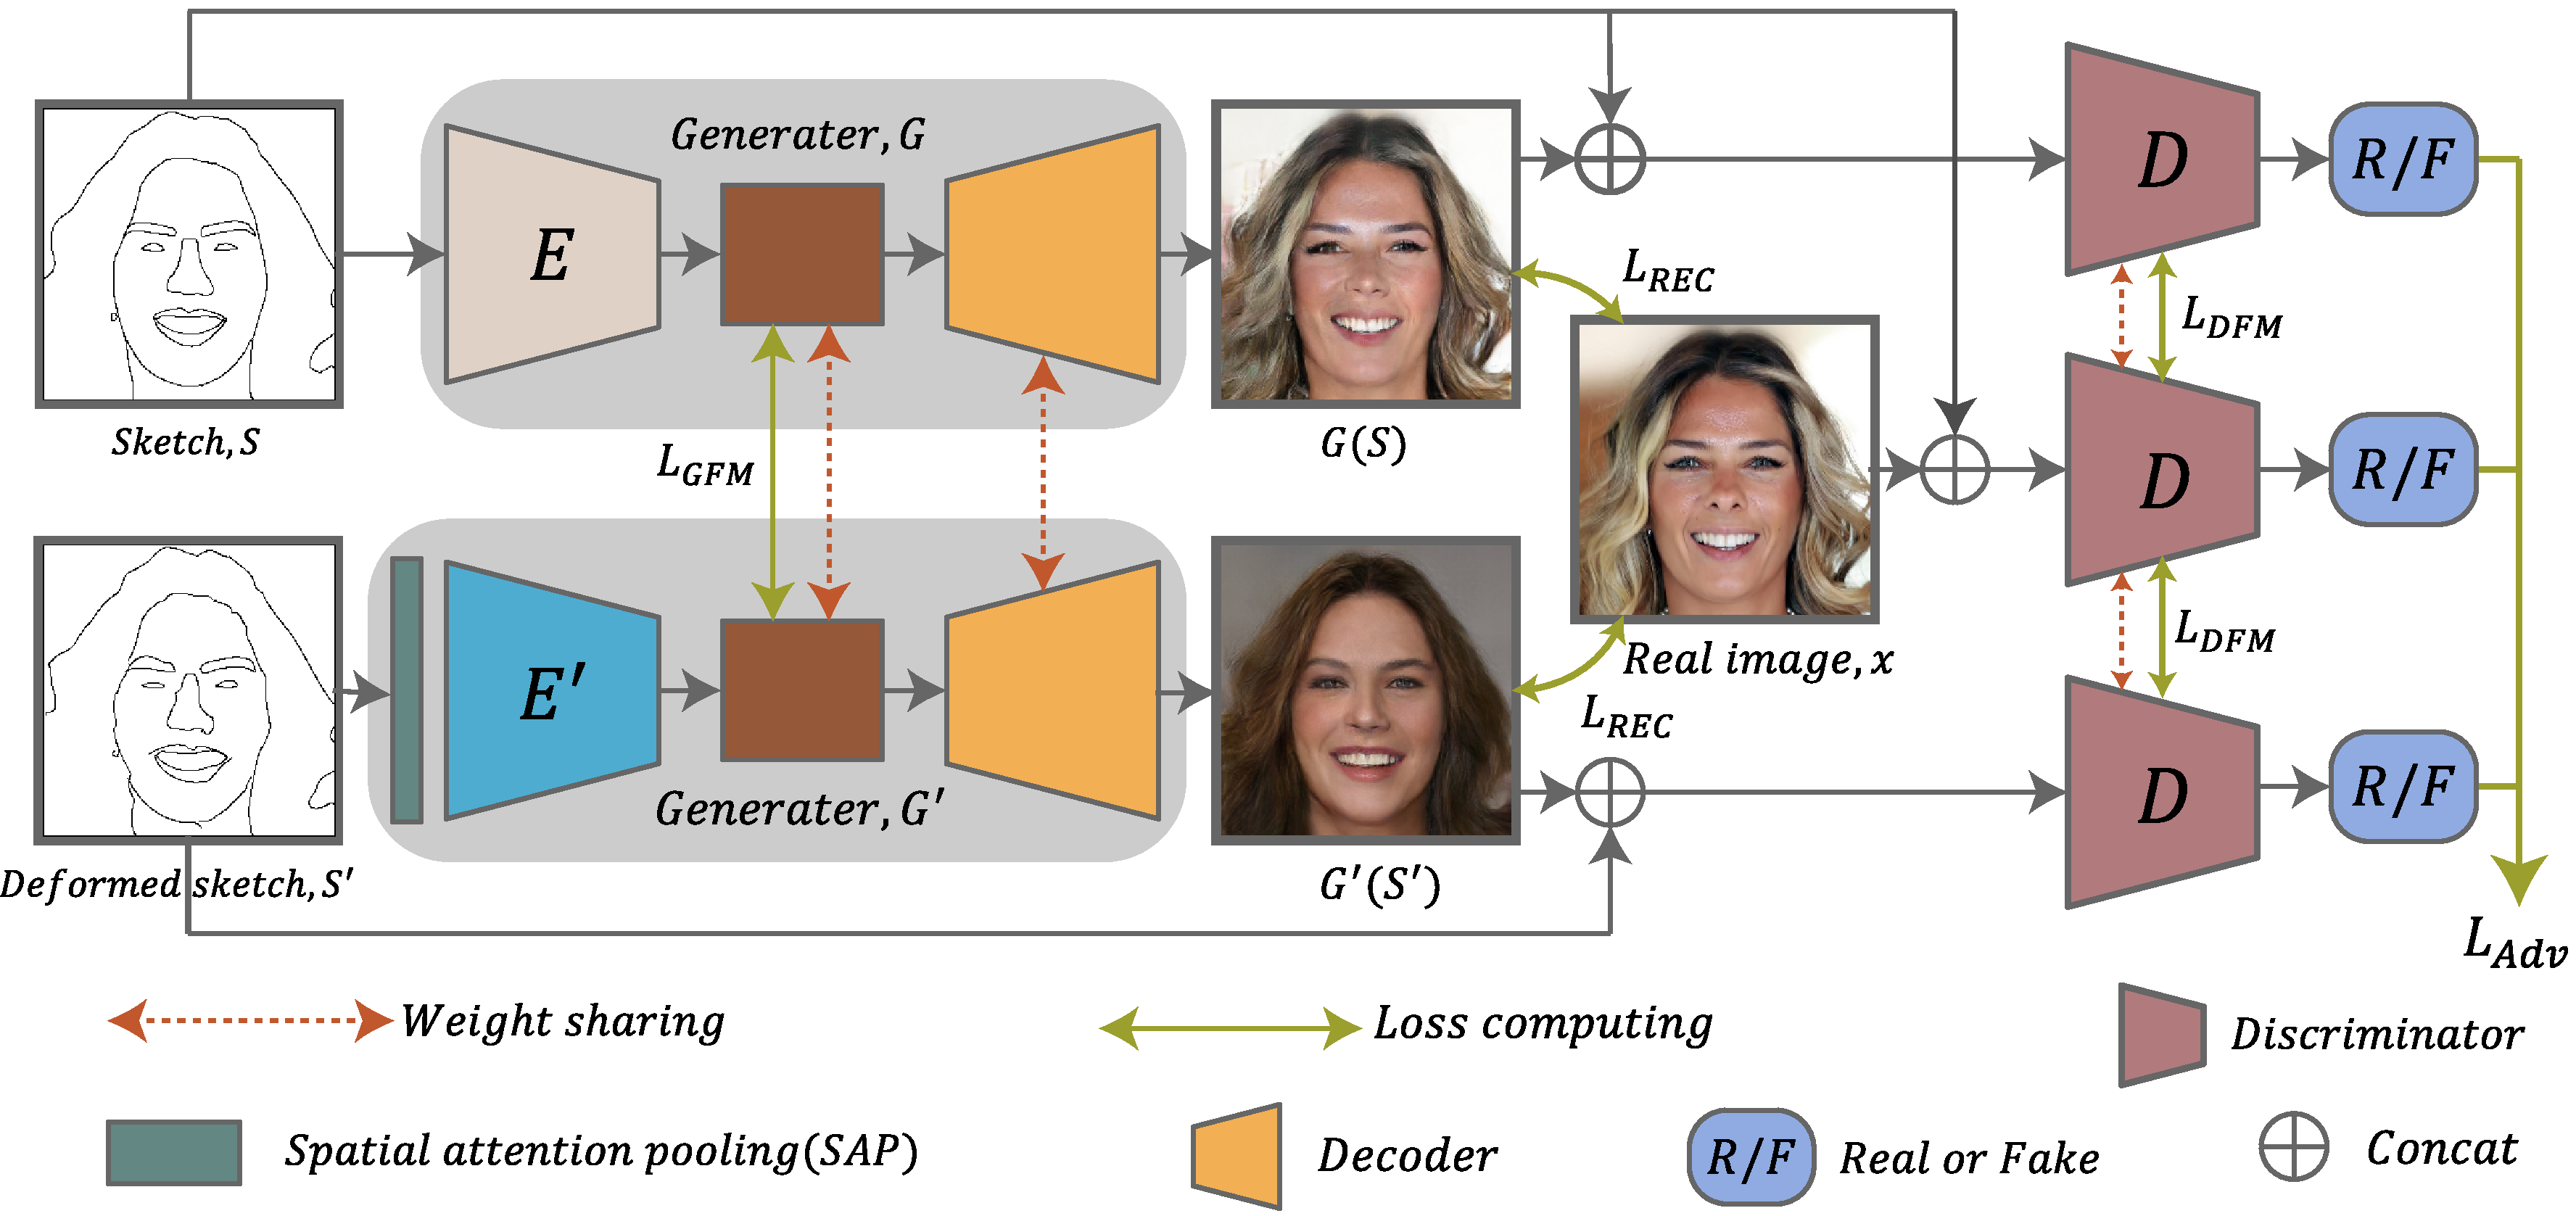
\includegraphics[width=0.9\textwidth]{figs/architecture}
	\caption{The architecture of our model.}
	\label{fig:architecture}
\end{figure*}
%
%%%%%%%%%%%%%%% Section Openning %%%%%%%%%%%%%%%%%%%%%%%%%%%%%%%%
In this paper, we propose a sketch-to-photo translation model that is robust to hand-drawn sketches. In order to handle hand-drawn sketches, we design a novel spatial attention pooling (SAP) module to adaptively adjust the spatial-variant balance between \textit{the realism} of the synthesized face image and \textit{the correspondence} between input sketch and the edges in synthesized image. 
We arrange this section as follow. We first introduce the dataset we construct for our model in Subsection~\ref{subsec:algorithm_data}.
Then we describe the architecture of our model in Subsection~\ref{subsec:algorithm_overview} and the proposed SAP in Subsection~\ref{subsec:algorithm_sap}.
At last we discuss losses applied in our model in Subsection~\ref{subsec:algorithm_loss} and the multi-stage training schedule in Subsection~\ref{subsec:algorithm_training}.




%%%%%%%%%%%%%% Face Sketches and Stroke Deformation  %%%%%%%%%%%%%%%%%%%%%%%%%%%%%%%%%%%%%%%
\subsection{Face Sketches and Stroke Deformation}
\label{subsec:algorithm_data}
% !TeX root = SketchFace.tex


Paired face sketch-photo dataset is required for supervised sketch-to-face translation methods.
Since there exits no large-scale paired face sketch dataset, the training face sketches used by existing methods are generated from face image dataset, e.g. CelebA-HQ face dataset, using edge detection algorithm such as HED~\cite{HED}.
%
However, the sketches generated by edge detection algorithm are sometimes incomplete or \td{other problems}. 
\td{Discuss the advance of make-edges over edge maps and contours}
\cxj{I would say the edge maps are quite different from handdrawn sketches, not because of the incompleteness.}
\rmv{ Although CSAGAN~\cite{CSAGAM} applied self-attention mechanism to alleviate the incompleteness problem, the others remains. Therefore we use another method to generate clearer and complete sketches from face images.}

~\cite{pix2pixHD} introduce another method to generate sketches from face images. Given a face image, the face landmarks are detected using an off-shelf landmark detection model. A new kind of sketch, denoted as \textit{face contour}, is obtained by connect specific landmarks. Sketch-to-face model trained by face contour fail to generalize to hand-drawn sketches with hair, wrinkles or beard. 

The CelebAMask-HQ dataset~\cite{CelebAMask-HQ} provides a face semantic map for each face image in CelebA-HQ dataset. We basically use the boundary map of the semantic map as the sketch of the corresponding face image. Figure~\ref{fig:sketch_data} shows an example of comparison between a sketch generated by edge detector, a face contour and a sketch generated from semantic boundary.
%


\paragraph{Stroke Deformation}
A shortcut of sketches generated from semantic boundary (and those generated by edge detector) is the lines of sketches are perfectly aligned to edges of the corresponding face images. In order to break the edge-alignment and mimic the hand-drawn sketches, we apply a deformation to the lines, similar to that in FaceShop~\cite{FaceShop}. Specifically, we vectorize lines of each sketches using AutoTrace algorithm~\cite{AutoTrace}, and add an offset randomly selected from $[-d, d]^2$ to the control points and end points of the vectorized lines, where $d$ is the maximum offset and we set $d=11$ in our experiments.
%
Both the initial sketches generated from semantic boundary and deformed sketches are used as the input sketches to our model.


\begin{figure}
	\centering
	\vspace{1.0cm}
	\caption{Comparison between a sketch generated from edge detection and from semantic boundary.}
	\label{fig:sketch_data}
\end{figure}


%%% TODO: add semantic map 
\begin{figure}
	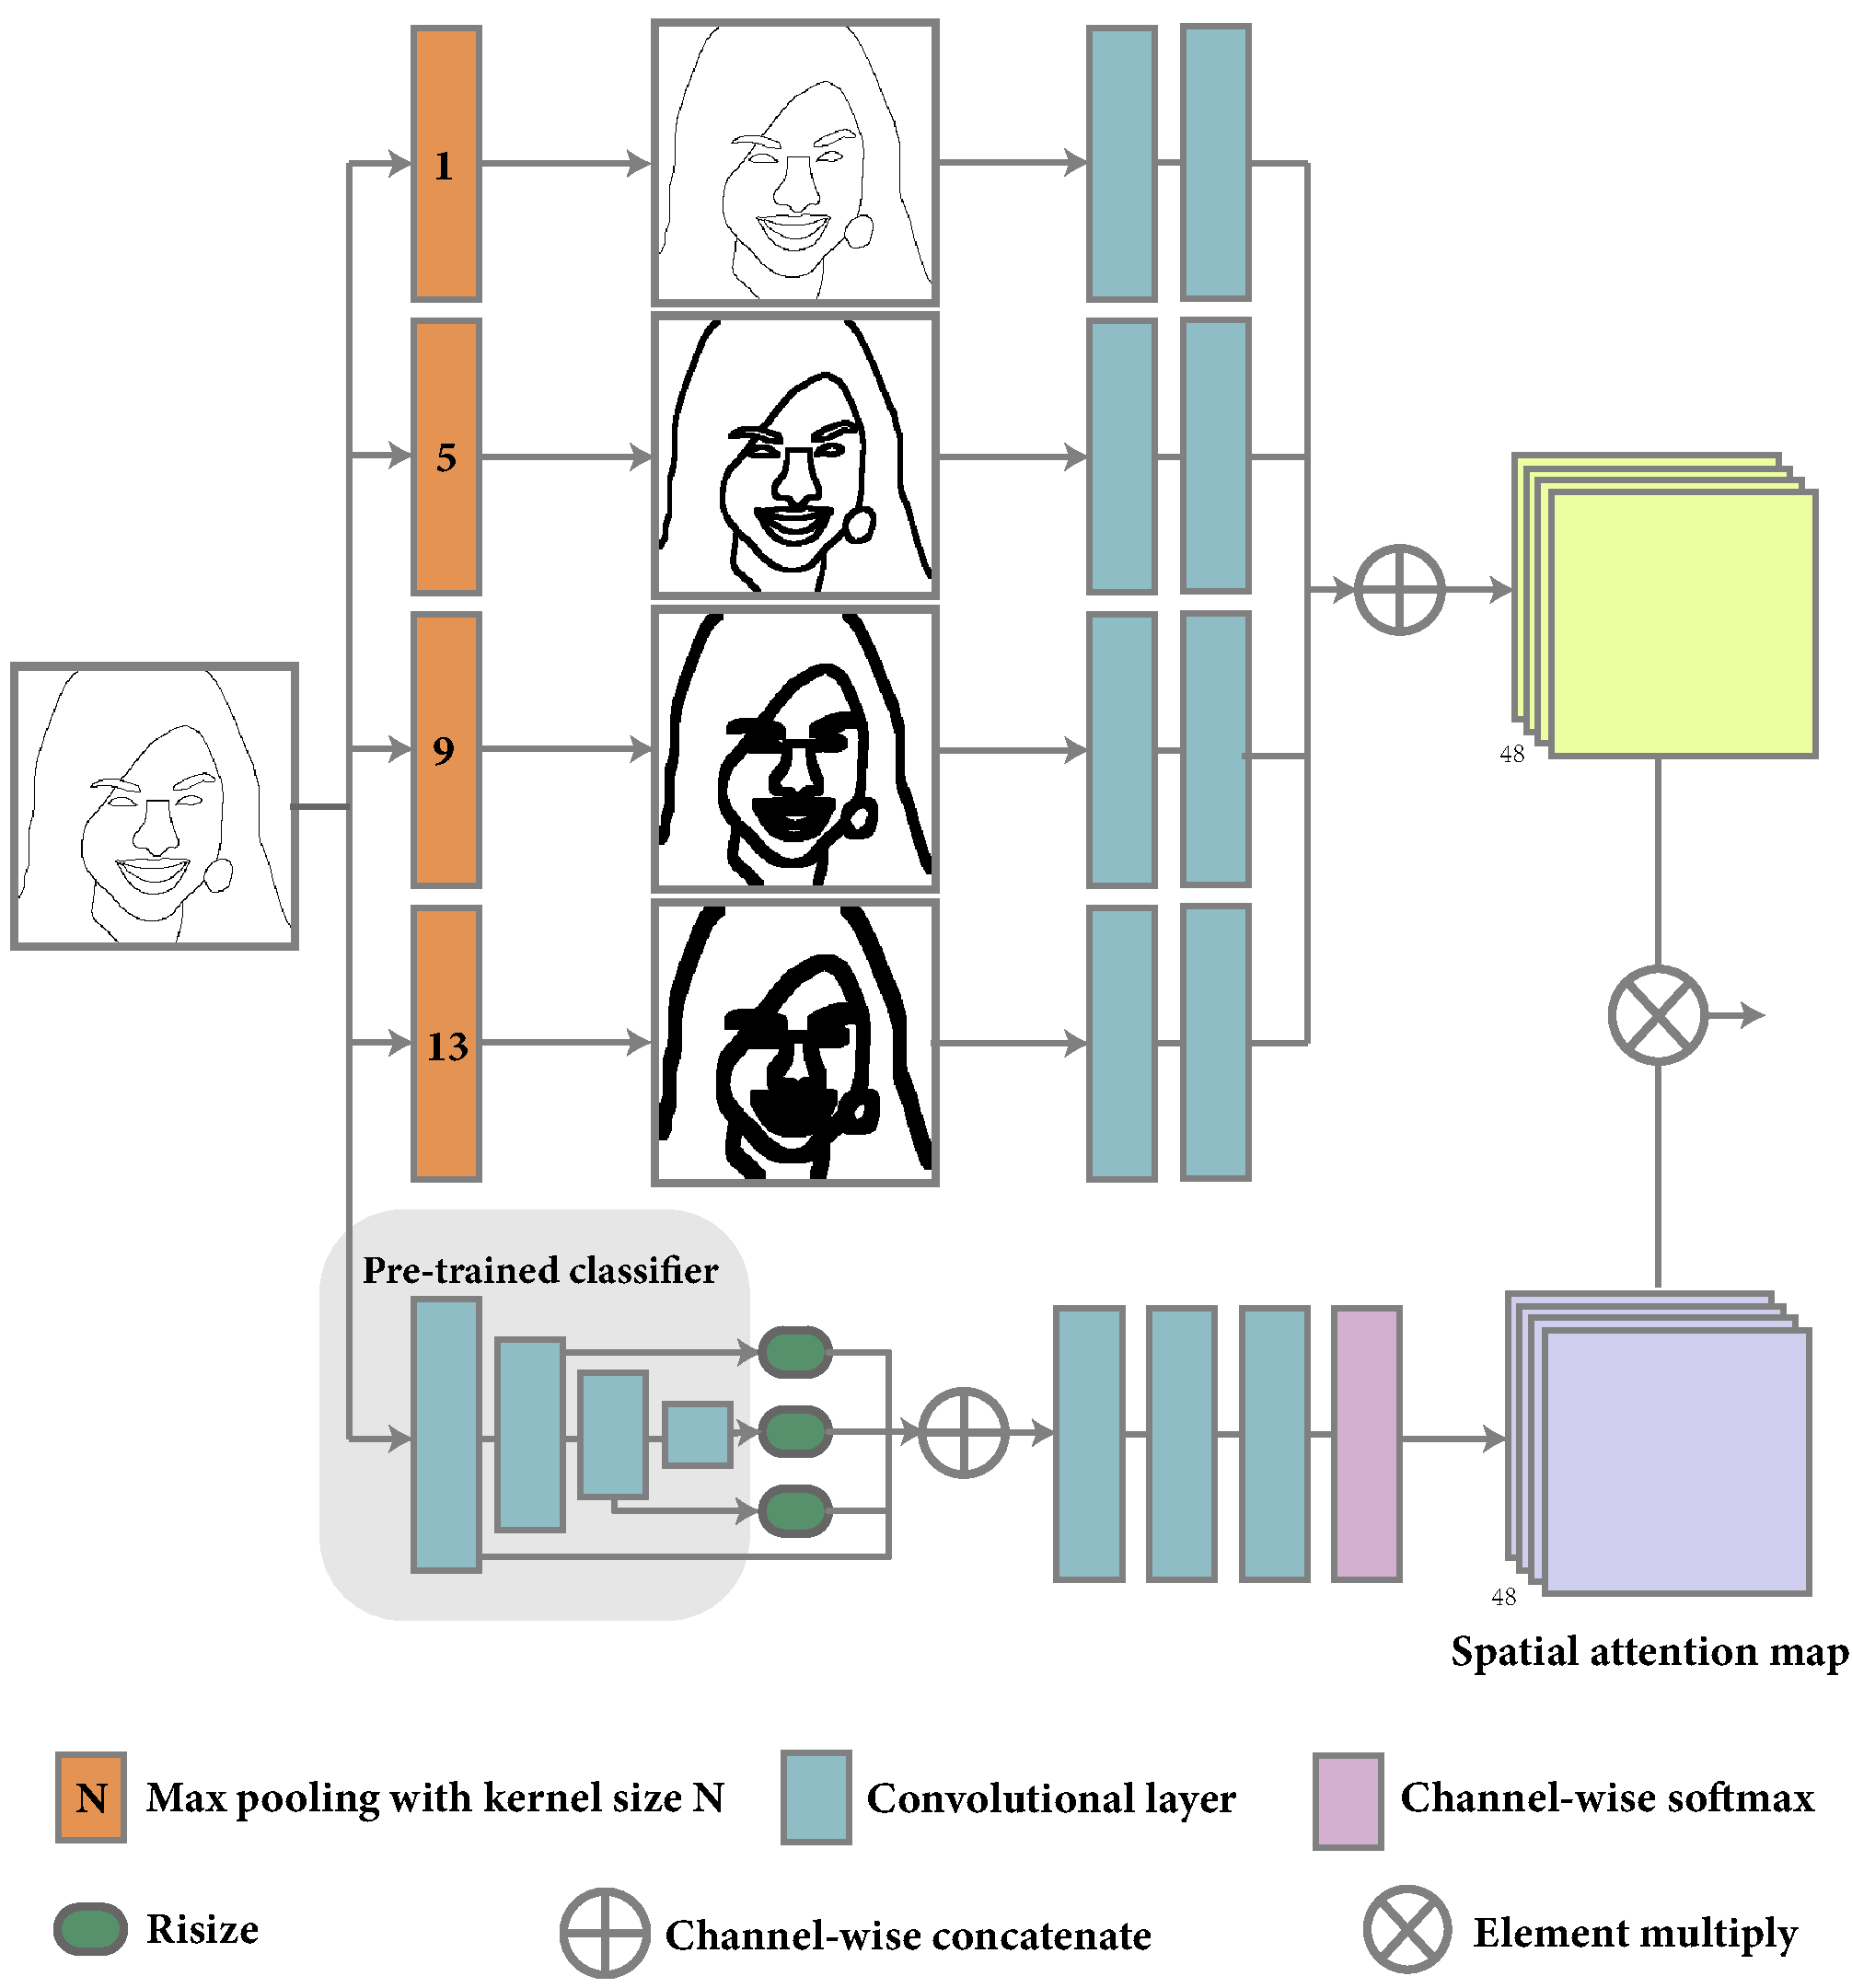
\includegraphics[width=\columnwidth]{figs/sap}
	\caption{Sap}
	\label{fig:sap}
\end{figure}
%
%%%%%%%%%%%%%% Overview  %%%%%%%%%%%%%%%%%%%%%%%%%%%%%%%%%%%%%%%
\subsection{Overview}
% !TeX root = SketchFace.tex
% 

The task of sketch-to-photo translation can be defined as looking for a generator $G(S)$ so that the generated image $G(S)$ from a hand-drawn sketch $S$ looks realistic and keeps the shape characteristics for the input sketch.
%
Existing image translation techniques train a neural network as the generator with paired of sketch and photo data $(\mathcal{S}, \mathcal{X})$.
%
Due to the scarcity of real hand-drawn sketches, existing techniques synthesize sketches in a certain style to approximate the sketch set $\mathcal{S}$ from face image set $\mathcal{X}$ to train their generator in an adversarial manner.
The synthesized sketches $\mathcal{S}_{syn}$ are usually well aligned with the face images and present different distributions from hand-drawn sketches $\mathcal{S}$.
These models typically fail to generalize to hand-drawn sketches by common users. 
%


We propose a novel network architecture with a specially designed training strategy to improve the capability of the sketch-based image generator.
%
Figure~\ref{fig:architecture} shows the overview of our method.
%
In order to synthesize a set of sketches that has similar distribution with hand-drawn sketches $\hdS$, we deform the edge-aligned sketches $\synS$ to generate a set of deformed sketches $\dfmS$ to augment the training set.
We propose a novel framework using dual generators from the edge-aligned sketches $\synS$ and the deformed sketches $\dfmS$ respectively.
%
$G_m$ is the main generator trained by deformed sketches $\dfmS$, aiming to generate plausible photo-realistic face images from unseen hand-drawn sketches in test stage. 
$G_a$ is an auxiliary generator trained with edge-aligned sketches whose goal is to guide $G_m$ to adaptively sense the line distortion in deformed sketches.
%
A spatial attention pooling module (SAP) is added before the encoder $E_m$ of $G_m$ to adjust the spatially varying balance between \textit{the realism} of generated images and \textit{the conformance} between the generated image and the input sketch. 
%



%%%%%%%%%%%%%% Spatial Attention Pooling  %%%%%%%%%%%%%%%%%%%%%%%%%%%%%%%%%%%%%%%
\subsection{Spatial Attention Pooling}
\label{subsec:algorithm_sap}
% !TeX root = SketchFace.tex

% 
\begin{figure}
	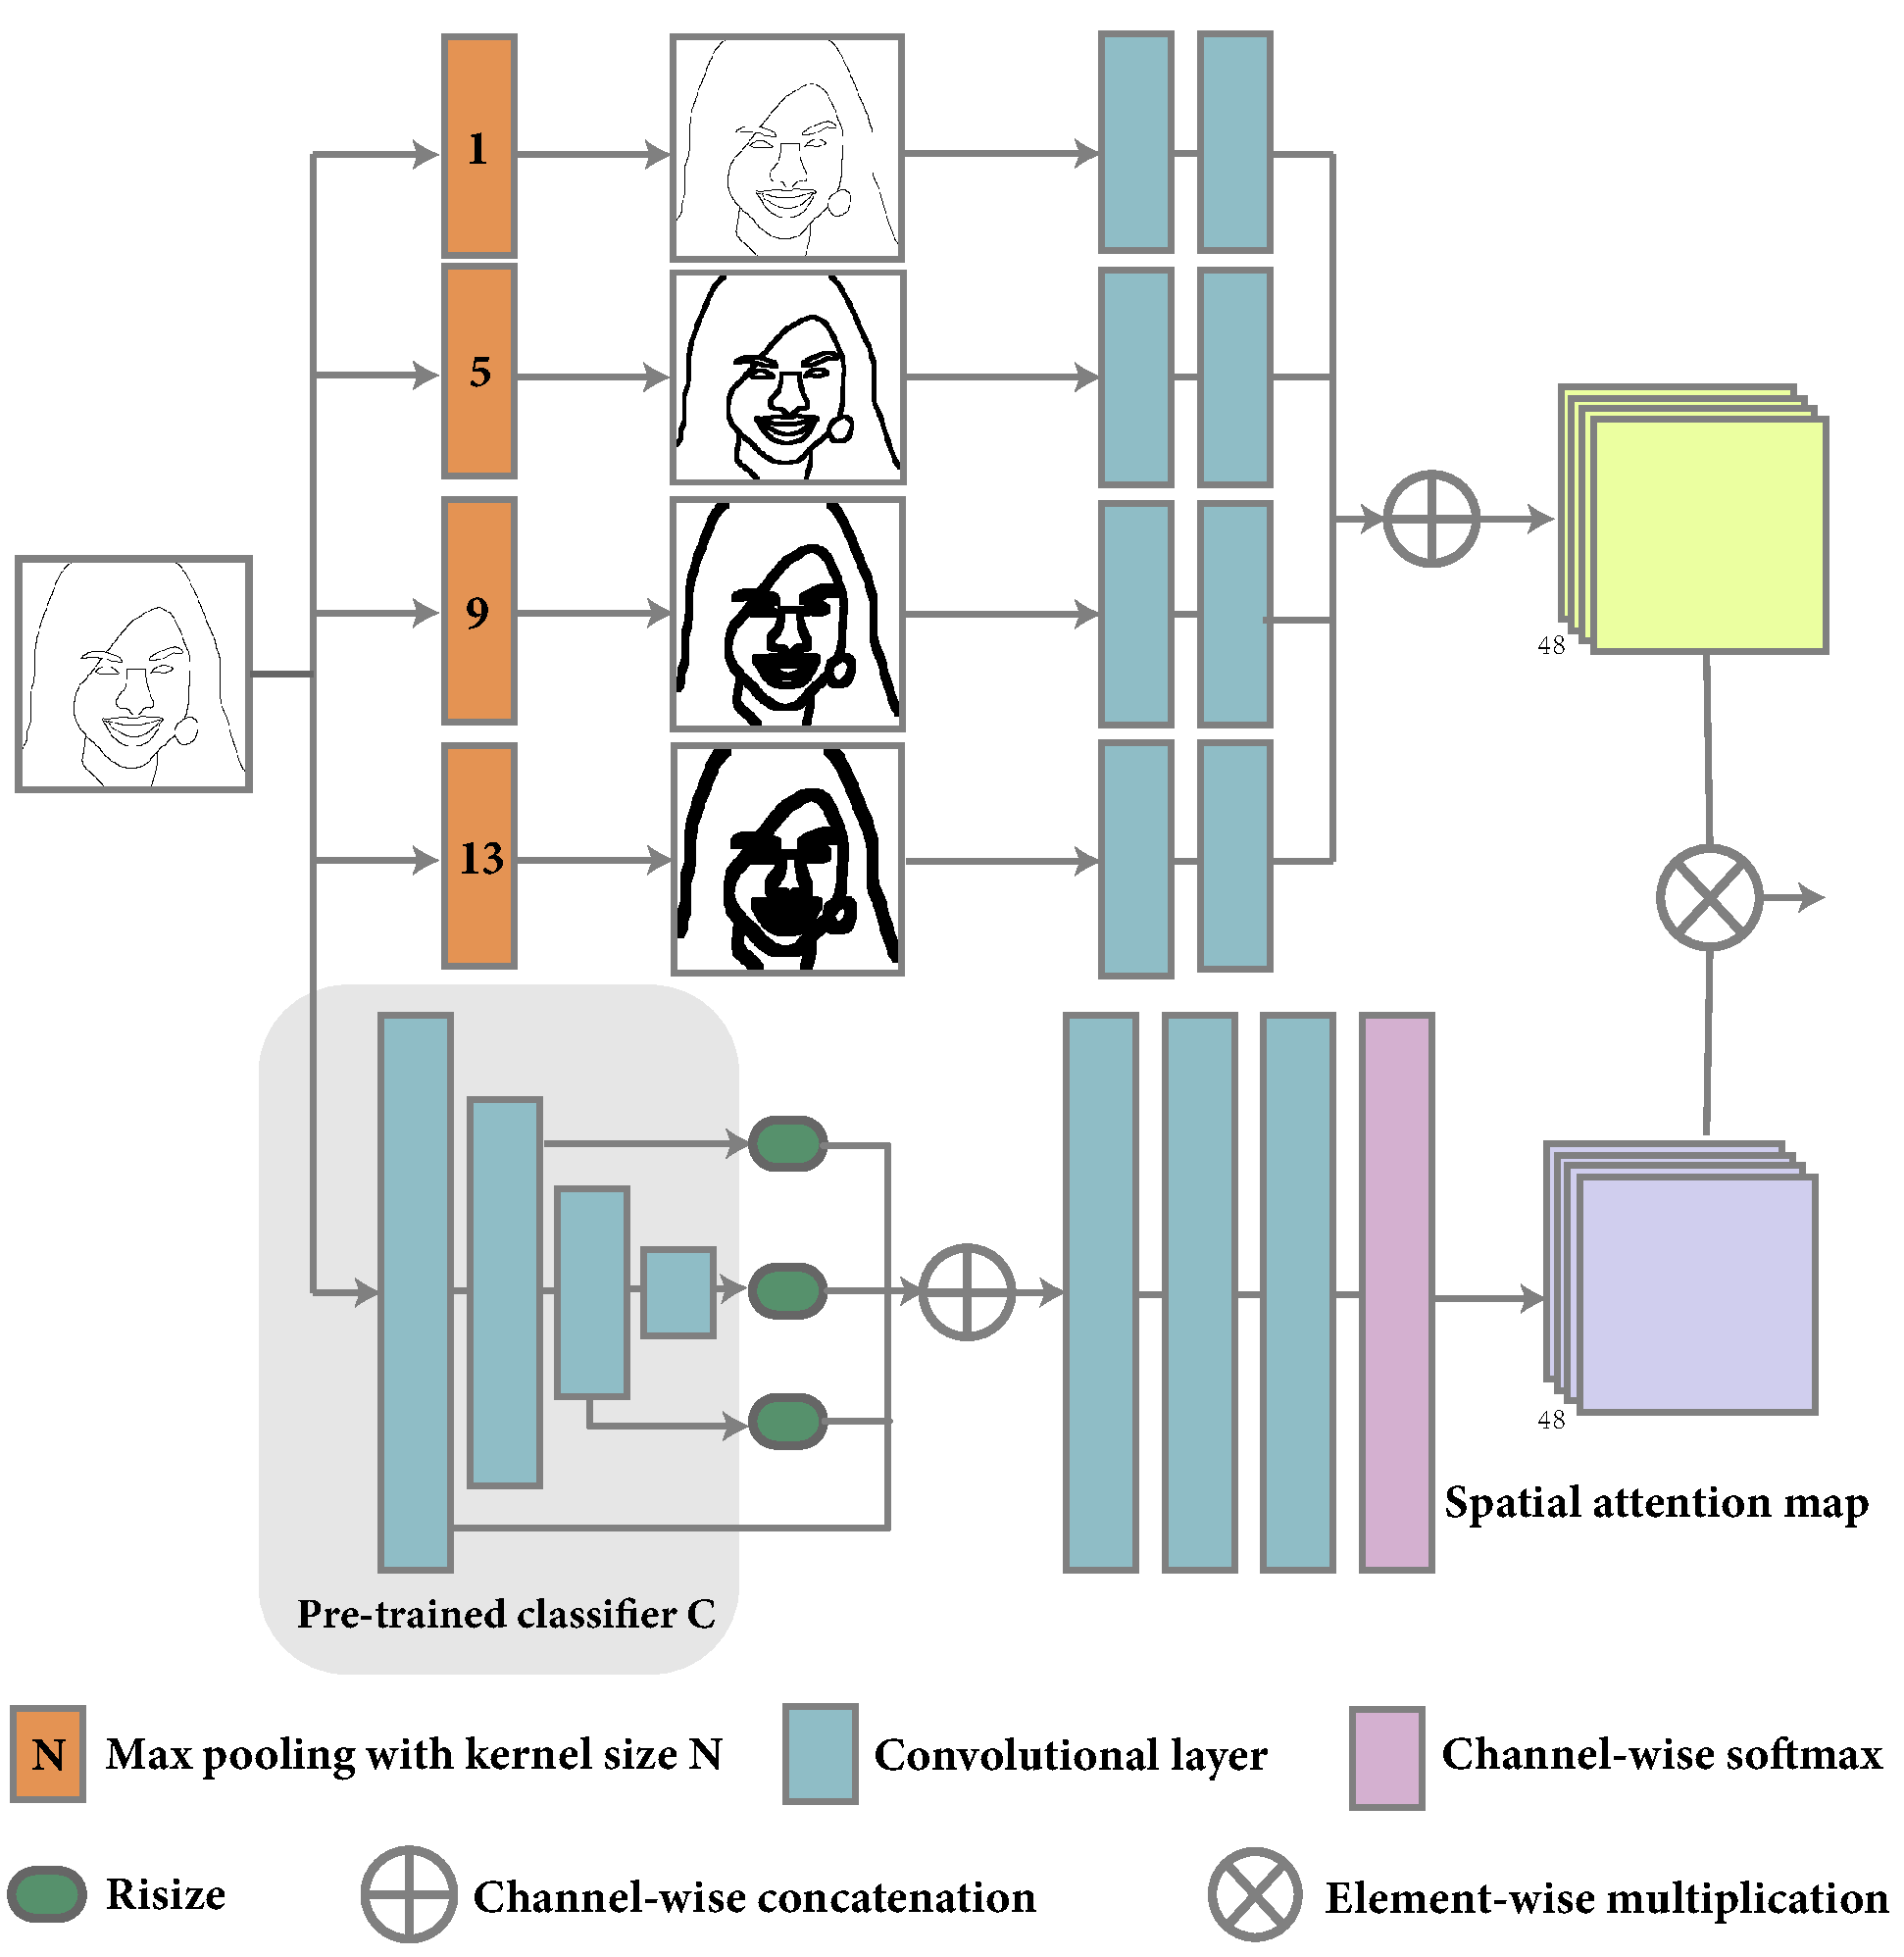
\includegraphics[width=\columnwidth]{figs/sap.png}
	\caption{Sap}
	\label{fig:sap}
\end{figure}
%

\subsubsection{Spatial Attention Pooling}
When the input hand-drawn sketch is not well-drawn, it is a trade-off between the realism of the output face image and the alignment between the input sketch and the output face image.
%
In order to alleviate the edge alignment between the input sketch and the output face image, we should relax the sharp sketch lines with one-pixel width.
\cxj{relax thin strokes to an ambiguity band with various width or uncertainty.}
One of the straightforward ways is to smooth the lines of sketches using image smoothing algorithm. 
Another is to dilate the sketch lines so that the widths of lines are of multiple pixels~\cite{DeepSurgery}.
\cxj{if it is not officially published, it is not necessary to cite it. but if our method performs better, then cite it and show comparison.}
However, the capacity of either the two hand-crafted ways above is limited, \td{because the uniform smoothness and the dilate radius for all positions of the whole sketch violate the unevenness of hand-drawn sketches on depicting different facial parts. }
%
We argue that the balance between the realism of the output face image and the alignment between the input sketch and the output face image differs from one position to another across the face image. Therefore, the smoothness or the dilation radius should be spatial-specific. 

Based on the discussion above, we propose a new module, called spatial attention pooling (SAP), to dilate the input sketch in a spacial-specific way. 
\cxj{I would not use 'dilate' since this simple word does not reveal the underlying discovery.}
%Let $\mathbf{r}=\{r_i | i=1,2,...,N_r\}$ be a set of dilation radius. 
Given an input sketch $S\in \real^{H\times W}$, we first pass it through $N_r$ pooling branches with different kernel sizes of $r_i, i=1,\ldots, N_r$ to get $\{P_{i}| i=1,\ldots,N_r\}$. 
Then we compute the spatial attention map $W\in \real^{N_r\times H\times W} $with $W = Softmax(f(s))$, where $f()$ is implemented with two convolutional layers. \cxj{$f(S)$ to extract low-level features from the input sketch?}
\cxj{It is not clear what is the motivation of computing the SA map $W$. It might be better to describe your idea of how to use $W$ with $P$ and then describe how to get $W$. }
%
A softmax layer which is computed over channels is added at the end of the convolutional layers, ensuring that for each position, the sum of weights of all channels equals to $1$. The output of SAP is computed as:
	
\begin{equation}
	SAP(s)=\sum_{i=1}^{N_r} W_i * P_{r_i}(s),
\end{equation}
%
where $W_i$ is the $i$th channel of $W$, \td{and $*$ is element-wise multiplication}.
\td{We show this idea in Fig.~\ref{fig:sap}.}








%%%%%%%%%%%%%% Losses  %%%%%%%%%%%%%%%%%%%%%%%%%%%%%%%%%%%%%%%
\subsection{Losses}
\label{subsec:algorithm_loss}
% !TeX root = SketchFace.tex

Our model consists of two generators, $G()$ for edge-aligned sketch $S$ and $G'()$ deform sketch $S'$, and one discriminator $D()$. Loss functions and objective of our model are discussed as follow.

\paragraph{Reconstruction Loss}
For either generator, a reconstruction loss is applied to guide the generated image to get close to its corresponding real image $x$.

\begin{equation}
\label{eqn:loss_rec}
\begin{aligned}
\mathcal{L}_{Rec}(G, G') &=\mathbb{E}_{(S, x)\sim p_{data}(S,x)\|G(S) - x\|_1} \\
&+ \mathbb{E}_{(S', x)\sim p_{data}(S',x)\|G'(S') - x\|_1},
\end{aligned}
\end{equation}

\paragraph{Adversarial Loss}
The multi-scale discriminator~\cite{pix2pixHD} $D$ consists of three sub-discriminators $D_i, i=1,2,3$.  The adversarial loss for $G$ and $D$ is defined as:
\begin{equation}
\label{eqn:new_loss_adv}
\begin{aligned}
\mathcal{L}_{adv}(G;D)&=\frac{1}{3}\sum_{i=1}^{3}E_{(\bm{S},\bm{x})\sim p_{data}(\bm{S},\bm{x})}\big[\log D_i(\bm{S},\bm{x})\big] \\
& + E_{\bm{x}\sim p_{data}(\bm{S})}\Big[\log \Big(1-D_i \big(\bm{S},G(\bm{S})\big)\Big)\Big].
\end{aligned}
\end{equation}
The adversarial loss for $G'$ and $D$ is defined similarly.

\paragraph{Discriminator Feature Matching Loss} Similar to pix2pixHD\cite{pix2pixHD} and lines2face~\cite{Lines2Face}, we use a discriminator feature matching loss as the perceptual loss, which is designed to minimize the error between generated image and real image in feature space. Here discriminator feature matching loss use the discriminator as the feature extractor. Let $D^q_i()$ be the output of $q$th layer in $D_i$. This loss for $G$ and $D$ is defined as:
\begin{equation}
\label{eqn:feature_matching_loss}
\mathcal{L}_{fm}(G)=\frac{1}{3N_Q}\mathbb{E}_{(\bm{S},\bm{x})\sim p_{data}(\bm{S},\bm{x})}\sum_{i=1}^{3}\sum_{q\in Q} \frac{1}{n_i^q} \|D^q_i(G(\bm{S}))-D^q_i(\bm{x})\|_1 ,
\end{equation}
where $Q$ is the selected layers of discriminator for computing this loss, $NQ$ is the number of elements in $Q$, $n^q_i$ is the number of elements in $D^q_i$.
Also, the discriminator feature matching loss for $G'$ and $D$ is defined similarly.

\paragraph{Generator Feature Matching Loss}
Similar to discriminator feature matching loss which is designed to minimize the error between generated image and real image in feature space, we propose a novel generator feature matching loss that aims to minimize the error between the presentations of $S$ and $S'$ in generator feature space. Let $G^t()$ and This loss is calculated as:

\begin{equation}
\label{eqn:loss_GFM}
\mathcal{L}_{GFM}(G, G')=\mathbb{E}_{(S, S')\sim p_{data}(S, S')} \frac{1}{N_T} \sum_{q\in Q}  \frac{1}{|G_q|} \|G_q(S)-G_q(\tilde{S}) \|_1,
\end{equation}


Let $G_q(\cdot)$ produces the feature maps of the $q$-th layer in the generator $G$.
%
Given an input sketch $S$ and the corresponding deformed sketch $\tilde{S}$, we compute the generator feature matching loss as:


%
where $|G_q|$ denotes the number of elements in $G_q(\cdot)$, $Q$ indicates a set of the selected generator layers for computing this loss and the size of $Q$ is $N_Q$. 
We select \td{the xxx layers} of the generator in our experiments.

Besides the generator feature matching loss $\mathcal{L}_{GFM}(G)$, for generator $G$ and multi-scale discriminator $D={D_k | k=1,2,...,N_D}$, the adversarial loss $\mathcal{L}_{GAN}(G, D)$ and the discriminator feature matching loss $\mathcal{L}_{DFM}(G, D)$ are computed as the same form as those in pix2pixHD~\cite{pix2pixHD}. \td{Discussion: add equations of these two losses or not}
%
The objective of the proposed model is:

\begin{equation}
	\label{eqn:new_minmax_game}
	\min_G \max_{D} \mathcal{L}_{GAN}(G, D)+\lambda \mathcal{L}_{DFM}(G, D) +\mu \mathcal{L}_{GFM}(G).
\end{equation}

where $\lambda$ and $\mu$ are the weights for balancing different losses. We set $\lambda=\td{xxx}$ and $\mu=\td{xxx}$ in our experiments.

%%%%%%%%%%%%%% Traning Schedule %%%%%%%%%%%%%%%%%%%%%%%%%%%%%%
\subsection{Training Schedule}
\label{subsec:algorithm_training}
% !TeX root = SketchFace.tex

In order to train our model more stably, we introduce a multi-stage training schedule. 
